\chapter{Chain Virtues}\label{chapter:virtues}

Now that we have developed the longest chain protocol and understand
what constitutes a chain, let's familiarize ourselves with executions
of this protocol, in honest and adversarial settings, by looking at
the combinatorial properties of chains.

\section{Transactions -- Blocks}

Before we get into the combinatorial properties of chains, let us spend a moment
comparing \emph{transactions} (Chapter~\ref{chapter:transaction}) and \emph{blocks}
(Chapters~\ref{chapter:blocks} and~\ref{chapter:chain}), to ensure
that we don't confuse the two and to built a high-level mental model of the
previous couple of chapters.

Recall from Chapter~\ref{chapter:transaction} that chain of transactions is what constitutes
a \emph{coin} (although this is not a formal notion, since coin provenance may not be uniquely
determinable because coins can be joined and split through transactions).
Anyone can create a transaction spending their own money instantaneously, because
they can easily create a signature. Long chains of such transactions can be created rapidly
from a low-end device, such as a mobile phone, with no significant mining power required.
On the other hand, no one can create a transaction that spends someone else's money,
because they don't hold the respective private key, no matter how much computational
power they have (within the bounds of our polynomial world). A chain of transaction
conveys no information about time taken.

As for blocks, creating them does not require producing any signatures, but does require
having a lot of computational power, and cannot be performed on a laptop or mobile phone.

A summary comparing blocks and transactions is shown in Table~\label{tbl:tx-block-compare}.
\emph{Time to create honest} describes the time needed to create a transaction spending my
own money (including double spending it) and the time needed for an honest party to mine an honest block.
\emph{Time to create adversarial} describes the time needed to create a transaction spending
someone else's money and the time needed for an adversarial party to mine an adversarial
block (for example containing a double spend). The last few rows summarize the inductive
process of validating a transaction and validating a block. For transaction validation, the
inductive base is the coinbase transaction, where money is generated and the Conservation Law
does not need to be verified, and neither do they need signatures.
The inductive hypothesis there is that we have a valid UTXO set,
and the inductive step involves updating the UTXO set by consuming and producing elements,
checking transaction signatures, and verifying the law of conservation. For block validation,
the inductive base is the genesis block, whose previd does not need to be checked. The inductive
hypothesis is that the previous chain up to $s$ has been validated, and the inductive step
involves checking the proof-of-work equation and validating the transactions within.

\begin{table}
\centering
\begin{tabular}{ |c|c|c| }
  \hline
  & \textbf{Transaction} & \textbf{Block} \\
  \hline
  \textbf{Time to create honest} & Instantaneous & Moderately hard \\
  \hline
  \textbf{Time to create adversarial} & Exponential & Moderately hard \\
  \hline
  \textbf{Inductive base} & Coinbase & $\mathcal{G}$ \\
  \hline
  \textbf{Inductive hypothesis} & Outpoint UTXO & Previous blockid ($s$) \\
  \hline
  \textbf{Inductive step} & \makecell{Update UTXO set \\ Check $\sigma$ \\ Conservation} & \makecell{$H(B) \leq T$ \\ Validate $\overline{x}$} \\
  \hline
\end{tabular}
\caption{A high-level comparison of the nature of transactions and blocks.}
\end{table}

Given this table, we can observe what protects a transaction in transit from being
altered. Imagine the adversary sitting in the middle of a gossip path on the network.
This adversary relays transactions and can modify them as they travel from one
end of the network to the other. If the adversary attempts to change a transaction's
data (such as the recipient), she will fail. The reason of failure is different for a
normal transaction and a coinbase transaction. When it comes to a normal transaction,
the polynomial adversary who attempts to change the recipient will fail because of the existential
unforgeability of the signature scheme. When it comes to a coinbase transaction,
these transactions are not signed, as they do not have any inputs. However, because
the coinbase transaction is always associated with a block, changing the coinbase
transaction invalidates the proof-of-work of the block the coinbase transaction is
included in. A coinbase transaction is never valid unless it accompanies a block.
The adversary would therefore need to solve the proof-of-work puzzle from scratch
in order to usurp this payment. While this is not impossible, it is moderately
difficult.

\section{Safety, Revisited}

When we gave the first intuitive definition of ledger safety in Definition~\ref{def:safety-informal}, we mandated that all honest parties
agree \emph{exactly} on their ledgers. Now that we've talked about network delays and arranged transactions into blocks, we see
that this will be impossible to achieve. In the best case scenario, we have a chain that is growing without any forks. Still, in this
case, if two honest parties $P_1, P_2$ both have a chain $\chain$, whenever $P_1$ mines a block $B$ on top of $\chain$, it will take
$\Delta$ time until $P_2$ receives this block and updates his ledger. Remember that the reported ledger of a party only includes the
transactions that have been confirmed into blocks.

We need to revise our safety definition to account for the fact that there can be discrepancies. We will accept that ledgers of honest
parties may disagree. However, we want the ledgers to be \emph{consistent} with one another: If one honest party has reported a transaction
at position $i$ in his ledger, then every other honest party must either have that same transaction at position $i$, or their ledger
must be shorter than $i$, indicating that the party has not yet decided which transaction to place at that location. However, it is imperative
that two different honest parties do not have different transactions at the same location. In different words, we want the ledger of
honest party $P_1$ and honest party $P_2$ to be \emph{prefixes} of one another, even if they are observed at different points in time.
Let's revise our \emph{ledger safety} virtue to state it formally.

\begin{definition}[Safety]\index{Safety}
  A protocol is \emph{safe} if
  for any two honest parties $P_1, P_2$ and any two times $r_1, r_2$, it holds that either
  $L^{P_1}_{r_1} \preccurlyeq L^{P_2}_{r_2}$ or $L^{P_2}_{r_2} \preccurlyeq L^{P_1}_{r_1}$.
\end{definition}

The notation $A \preccurlyeq B$ between two finite sequences $A$ and $B$ means that
$B[{:}|A|] = A$. An example of safe ledgers is illustrated in Figure~\ref{fig.safe-ledgers}.
The image shows the ledgers reported by all honest parties at potentially different points
in time. The same transaction is illustrated as a circle of the same color on different ledgers.
Not all parties have seen all transactions yet: Party $P_2$ has seen more transactions than
any other party, while $P_5$ has seen the fewest. At position $8$, only $P_2$ has seen the white
transaction, and every other party has not. However, if a transaction ever appears in position $8$
of any other honest party (illustrated as a dashed-line ghost transaction), it will be the same
exact transaction that party $P_2$ has seen at that position.

% TODO: show an example of unsafe ledgers in a similar fashion
\begin{figure}[h]
    \centering
    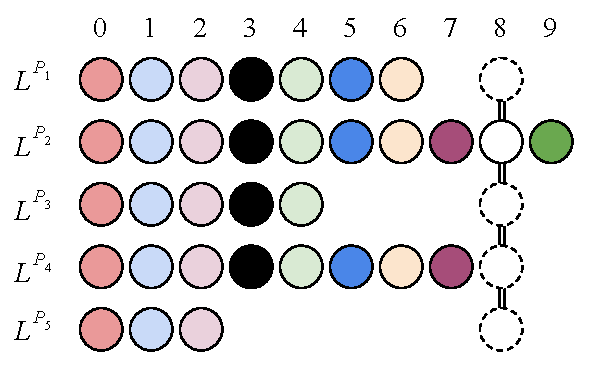
\includegraphics[width=0.65 \columnwidth,keepaspectratio]{figures/safe-ledgers.pdf}
    \caption{A god's eye view of the \emph{safe} ledgers of various honest parties at various moments in time.}
    \label{fig.safe-ledgers}
\end{figure}

Thinking back to the UTXO model, safety means that the transaction graph of one party is outdated, but not inconsistent, as compared
to the other party. In particular, if one party has confirmed a transaction $\tx$, then the other party cannot have confirmed, and can
never confirm, a transaction $\tx'$ which is a double spend of $\tx$. Let's try to understand why.

\begin{lemma}[Safe $\Rightarrow$ No double spend (informal)]
In a safe protocol that ensures transaction validity locally,
two honest parties can never confirm two conflicting transactions.
\end{lemma}
\begin{proof}
Suppose, towards a contradiction, that party $P_1$ at time $r_1$ has confirmed $\tx$. This means that $\tx$ appears in $P_1$'s
ledger $L^{P_1}_{r_1}$ at time $r_1$, and let's call $i$ the position of the transaction in the ledger: $\tx = L^{P_1}_{r_1}[i]$.
Additionally, party $P_2$ at time $r_2$ has confirmed $\tx'$, a conflicting transaction to $\tx$. Similarly, let $j$ be the index:
$\tx' = L^{P_2}_{r_2}[j]$. Now, if $i = j$, then this means that $\tx = \tx'$, which is a contradiction since these are conflicting.
If $i < j$, then by safety this means that $L^{P_2}_{r_2}[i] = L^{P_1}_{r_1}[i] = \tx$. But then, party $P_2$ has included
in his ledger \emph{both} $\tx$ at position $i$ \emph{and} $\tx'$ at position $j$. This is a contradiction, because the honest
party validates $\tx'$ before accepting it. Therefore, the two parties cannot have accepted conflicting transactions.
\end{proof}

This is a good sanity check that our definition of safety makes sense. Is this revised and precise, yet weaker, notion of ledger
safety achieved by our \emph{longest chain} construction? Not quite. The problem is that, as we saw in the previous chapter,
the chain may have \emph{temporary forks} even when no adversary is mining. Whenever the chain \emph{reorgs}, there is a
potential for safety loss. Consider the case illustrated in Figure~\ref{fig.reorg-safety-loss}. Imagine that honest party
$P_1$ had initially adopted the chain whose tip is block $6$ and contains the top (white) transaction $\tx$. In the meantime
party $P_2$, who has not seen block $6$ yet, is still mining on top of block $4$. If party $P_2$ successfully mines block
$5$, he can include a double spending transaction in it, the bottom (black) transaction $\tx'$, conflicting with $\tx$.
Now the two chains at blocks $5$ and $6$ are at a tie. The tie will be broken when the next proof-of-work
is found (block $7$) and one branch becomes longer; the nodes that were working on the other
(block $6$) branch will then switch to the longer one. If we now compare the ledger reported by party $P_1$ when he
had adopted block $6$ and the ledger reported by party $P_2$ when he had block $7$, we see that the
ledgers obtained by \emph{reading} these two chains are mutually unsafe.

\begin{figure}[h]
    \centering
    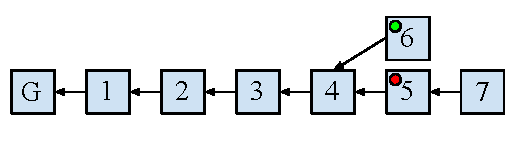
\includegraphics[width=0.5 \columnwidth,keepaspectratio]{figures/reorg-safety-loss.pdf}
    \caption{A chain reorg during a temporary fork causes a safety loss.}
    \label{fig.reorg-safety-loss}
\end{figure}

We will have to revise our \emph{reading rule} to account for these temporary forks.

\section{Honest Convergence}
We now argue that, in a correctly parametrized system, temporary forks will generally be short.
Let us initially analyze this claim in the setting where every miner is honest.

\begin{figure}[h]
    \centering
    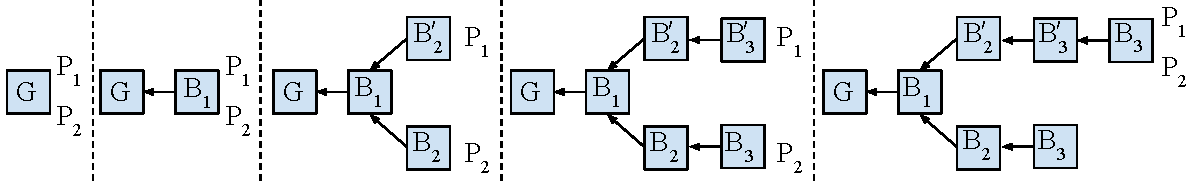
\includegraphics[width=\columnwidth,keepaspectratio]{figures/mining-factions.pdf}
    \caption{The timeline of two honest parties $P_1$ and $P_2$ mining in a way that causes
             the honest population to temporarily split between two factions.}
    \label{fig.mining-factions}
\end{figure}

Before we give a proof of this, let us think through an example of chain divergence and convergence.
It is illustrated in Figure~\ref{fig.mining-factions}.
Initially, all honest parties are mining on top of genesis $\mathcal{G}$. If it happens that an honest party
gets a block $B_1$, and broadcasts it to the rest of the network, this block will arrive at the doorstep of every other honest
party within time $\Delta$. If no other block was mined during that time, now all honest parties will
switch to $B_1$. Convergence is maintained. This can continue happening, and the chain will
keep growing, with all parties agreeing on one tip (with potentially a small delay). Now, the divergence
case can happen when two honest parties mine a block almost simultaneously: First, one honest party
mines a block $B_2$ on top of block $B_1$ and broadcasts it to the network. But before $\Delta$ time has
elapsed, a second honest party mines block $B_2'$. The block $B_2'$ will also be on top of block $B_1$,
as the second party has not received $B_2$ yet. At this point, two different chains, with tips $B_2$
and $B_2'$ respectively, exist and have the same length. Now the honest mining power is split into
two factions: Some honest nodes have seen $B_2$ first, whereas other honest nodes have seen $B_2'$
first, so some honest nodes are trying to extend $B_2$ and some others are trying to extend $B_2'$.
These factions may hold different, or similar, portions of compute. Now it's possible that an
honest party mines another block $B_3$ extending $B_2$. The party broadcasts it to the network,
but, before $\Delta$ time has elapsed, another party, who was mining on top of $B_2'$, also mines
block $B_3'$ which extends $B_2'$. Again the honest parties are split between two different chains
of the same length. This situation can continue. At some point, an honest party will mine a block
$B$ and broadcast it to the network, but no other block will be mined within $\Delta$ time. At
this point, every honest party will switch to block $B$. This is the convergence opportunity.

The idea is that, if we choose $T$ appropriately, then convergence opportunities will happen regularly.
Once a convergence opportunity happens, if there is no adversarial miner, the honest parties will converge into
one chain.

\begin{lemma}[Honest Convergence]\label{lem:honest-convergence}
    In a setting where only honest parties are mining, exactly $\Delta$ time after every convergence
    opportunity, all honest parties will hold the same chain.
\end{lemma}
\begin{proof}
    Consider an arbitrary convergence opportunity producing block $B$ occurring at time $r$.
    Since the convergence opportunity is $\Delta$ separated from every \emph{preceding} successful query,
    and all successful queries are honest and broadcast to the network, all honest parties will
    have seen all the blocks produced so far (because they all happen prior to $r - \Delta$ and it
    takes at most $\Delta$ time to receive the message containing those blocks).
    Therefore, the honest party who mined $B$
    will be mining on top of the longest chain among all. This means
    that, at time $r$, the block $B$ has a height larger than any other
    block. Because the miner is honest, he broadcasts $B$, and it is received by all honest parties within $\Delta$
    time. Since the convergence opportunity is $\Delta$ separated from every \emph{succeeding} successful
    query, no other blocks are mined or during the time interval $r \ldots r + \Delta$.
    At time $r + \Delta$, every honest party has received $B$ and adopted it since it is
    the longest chain. At this point, all the honest parties agree on their chains.
\end{proof}

\begin{figure}[h]
    \centering
    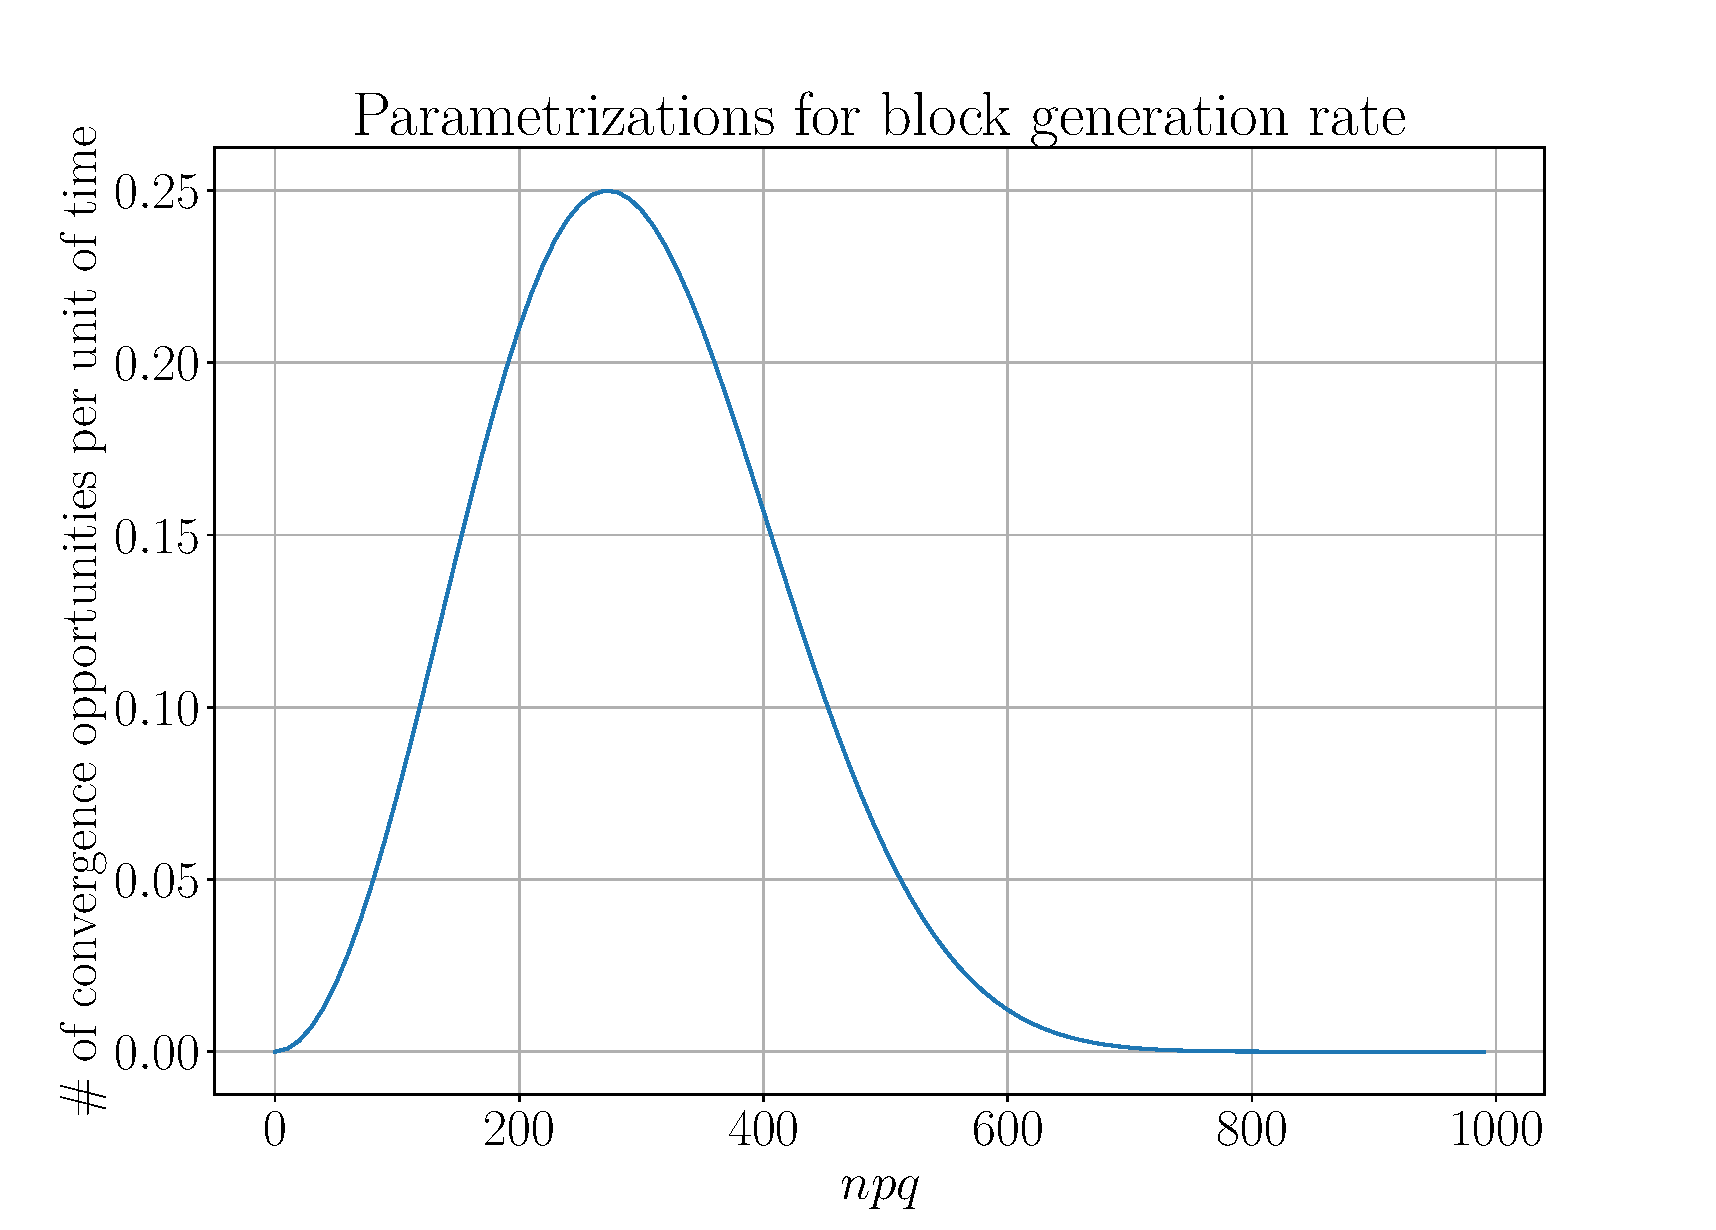
\includegraphics[width=0.8 \columnwidth,keepaspectratio]{figures/p-vs-convergence-opportunities.pdf}
    \caption{The relationship between the expected block production rate $nqp$
             and the density of convergence opportunities.}
    \label{fig.p-vs-convergence-opportunities}
\end{figure}

% TODO: Consider moving this paragraph to after the Nakamoto race section
In other words, convergence opportunities really do lead to convergence in honest executions.
But will convergence opportunities happen often, as we are hoping?
This depends on the choice of parameter $T$,
which affects $p = \frac{T}{2^\kappa}$, and it should be tuned based on our best guess for
$n, q, \Delta$ we have
for the network. Let us visualize the effect that the expected block production rate $nqp$
(if all $n$ parties are actively mining), of which we can tweak $p$, has on the density of
convergence opportunities in the unit of time. Their relationship is visualized in
Figure~\ref{fig.p-vs-convergence-opportunities}. As you can see in this graph, there's a
sweet spot for the expected block production rate that maximizes convergence opportunities.
If we make block production rate too slow (left side of the plot), convergence opportunity
density in the unit of time drops. The reason is that, while almost all successful queries
are convergence opportunities, they are very rare in time. On the other hand, if we make
block production rate too quick (right side of the plot), while successful queries are dense
in time, convergence opportunities are rare, because successful queries clash with one another
and there is no sufficient $\Delta$ separation between them. It is our task to design a system
that \emph{always} remains within the realm of good density of convergence opportunities.
A system that produces blocks
very fast may appear to have a high throughput of ``transactions per second'', but this
misconfiguration can be leading to insecurity, because throughput has been increased to
the detriment of convergence opportunity density. Any claims of blockchain performance
must always be accompanied by how the parametrization that achieves that performance affects
the security of the network.

\section{Common Prefix}
Under a correct parametrization of the system, we have now developed some intuition that
temporary forks will be short, at least as long as everyone is honest. These forks may
develop some length, but soon enough, a convergence opportunity will arise. At that point,
all forks apart from one will be abandoned, and the honest parties will convergence on
one chain. It takes time to mine a temporary fork of longer length.
Because convergence opportunities will occur often (we will
calculate precisely how often in Chapter~\ref{chapter:earnest2}),
there is not enough time to build long temporary forks. Our blocktrees will look roughly
like Figure~\ref{fig.honest-chain-common-prefix}.

\begin{figure}[h]
    \centering
    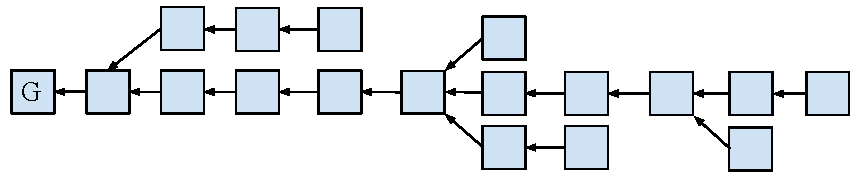
\includegraphics[width=0.7 \columnwidth,keepaspectratio]{figures/honest-chain-common-prefix.pdf}
    \caption{An honest execution with some short temporary forks.}
    \label{fig.honest-chain-common-prefix}
\end{figure}

We will now define a parameter $k \in \mathbb{N}$ that specifies our belief of how long
these temporary forks can get. Our hope is that there will be no temporary fork longer than
$k$. If this is respected, we will be able to ensure safety. We call this virtue of chains
the \emph{Common Prefix} virtue.

\begin{definition}[Common Prefix]\index{Common Prefix}
  A system is said to satisfy \emph{Common Prefix} with parameter $k \in \mathbb{N}$ if
  for all honest parties $P_1, P_2$ and for all times $r_1 \leq r_2$, the chains adopted
  by the honest parties satisfy the property that

  \[
    \chain^{P_1}_{r_1}[{:}-k] \preceq \chain^{P_2}_{r_2}\,.
  \]
\end{definition}

This property is telling us that temporary forks do not extend beyond $k$ blocks long.
For example, the Common Prefix virtue holds in Figure~\ref{fig.honest-chain-common-prefix}
with parameter $k = 3$, because temporary forks are at most $3$ blocks long. The precise
statement of the virtue states that, if we take the chains adopted by two honest parties
at the same point in time, and we \emph{chop off} $k$ blocks from the end of the chain of
the chain of one party, we get a \emph{prefix} of the chain of the other party. In other
words, the two honest parties' chains share a long common prefix, and their different
suffixes can only be up to $k$ blocks long.
This further holds if we take chains of different parties at different points in time.
In that case, we have to
make sure we chop off blocks from the \emph{old} chain to find that it is a prefix of the \emph{newer}
chain. The property also applies when $P_1 = P_2$, in which case it is telling us that
a particular honest party cannot perform chain reorgs more than $k$ blocks deep.

If this virtue holds, and we can know a $k$ parameter that bounds all of our temporary
forks, we can modify the \emph{read} functionality to achieve safety. Instead of reporting
as \emph{confirmed} the transactions that are in our adopted chain $\chain$, we report as \emph{confirmed}
the transactions that are within $\chain[{:}-k]$, our chain with the last $k$ blocks chopped
off. If the Common Prefix virtue holds, we know that the blocks in $\chain[{:}-k]$ will never
be abandoned in the future.

Our new, and final, confirmation rule, is illustrated in
Algorithm~\ref{alg.read-stable}. Compare this rule to Algorithm~\ref{alg.read-naive} of
the previous chapter. The only difference is that we have replaced $\chain$ with $\chain[{:}-k]$.
The portion $\chain[{:}-k]$ is called the \emph{stable} part of the chain, because we
are assured it will not change.

\import{./}{algorithms/alg.read-stable}

We have finally achieved safety. This is captured in the following theorem, whose proof we will
complete in Chapter~\ref{chapter:earnest2}.

\glsxtrnewsymbol[description={common prefix}]{common prefix}{$k$}\glsadd{common prefix}
\begin{theorem}[Common Prefix $\Rightarrow$ Safety (informal)]
    If the blocktree satisfies Common Prefix with parameter $k$, then the longest chain protocol
    with the $k$-confirmation rule is safe.
\end{theorem}

Note the effect of $k$ on the protocol. If we make $k$ too small, then we risk Common Prefix
being violated, and safety becoming jeopardized. If we make $k$ too large, then liveness will
deteriorate. Similarly to how we must tune the $T$ parameter appropriately to balance safety
and liveness, so we must also tune the Common Prefix parameter $k$.

With this small change to the implementation of \emph{read}, our protocol is finally complete.
We have created a secure cryptocurrency. The rest of this book will be devoted to studying the
various properties of our construction, augmenting it so that it remains secure in different models,
and optimizing it. However, the central construction is done.

\section{The Nakamoto Race}

We now bring Eve, our double spending adversary, back into the picture. Eve has picked up her game.
Instead of stealing a cup of coffee, she's now attempting to steal a brand new car!
However, she's now up against our $k$-confirmation protocol and must work a lot harder than before. The attack is
pictured in Figure~\ref{fig.nakamoto-race}. Initially, all parties have converged on some block $B$.
Eve first creates two conflicting transactions
$\tx$ (the white transaction on the bottom chain) and $\tx'$ (the black transaction on the top chain).
In this case $\tx$ is paying for the brand new car, whereas $\tx'$ is spending the same
output and handing the money back to herself. She broadcasts $\tx$ to the network, hoping that
it will become confirmed by the honest parties and observed by the car dealer so that she can be handed
the car. The honest parties receive $\tx$ from the network and faithfully include it into their mempool.
At this point, Eve starts \emph{secretly} mining on her own on the top (red) fork, while the honest
parties are mining on the bottom blue fork. The honest parties do not mine on top of adversarial blocks,
because Eve does not broadcast these blocks to the network.
Eventually, the honest parties mine a block containing $\tx$ (the block on the lower fork containing the
white transaction). But the car dealer will not see $\tx$ marked as \emph{confirmed} in his wallet before it is
buried under $k$ blocks, so Eve must wait. Eve allows the honest parties to keep mining on the
bottom chain until $k$ blocks have been mined on top of the transaction and the transaction appears
as confirmed. That's when the car dealer hands over the car to Eve. She takes the car and drives away.
In the meantime, Eve has been mining on the top fork during for all this time. If at this time she has
managed to create a longer chain than what the honest parties have already adopted, she reveal this
chain to the network by broadcasting it. Then, every honest party will reorg their chains and switch
to Eve's chain. She will take her money back, and she will have gotten away with the car.

\begin{figure}[h]
    \centering
    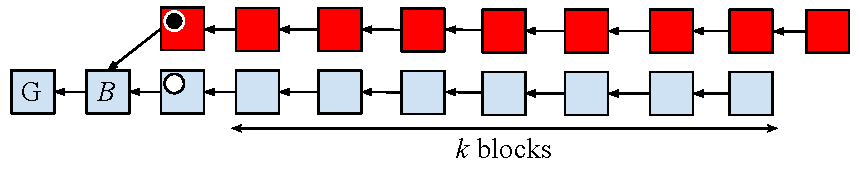
\includegraphics[width=0.7 \columnwidth,keepaspectratio]{figures/nakamoto-race.pdf}
    \caption{The Nakamoto Race.}
    \label{fig.nakamoto-race}
\end{figure}

To see when this attack is successful, we argue as follows. As soon as block $B$ was found and broadcast
to the network at some time $r$, a \emph{race} began between the honest parties and the adversary:
the so-called \emph{Nakamoto Race}\index{Nakamoto Race}.
This race concludes as soon as the honest parties have mined $k + 1$ blocks on the bottom fork.
It is pointless for Eve to broadcast her top fork if the bottom fork does not have $k + 1$ blocks
in it, because this will simply leave her car-purchasing transaction unconfirmed and Eve carless.
Because blockchains take time to produce, it will take time to mine these $k$ blocks. In order for
Eve to win she must have mined more blocks than the honest parties within that time window. Whether
she is successful in doing this depends on whether she has more mining power than the honest
parties or not. If Eve has less mining power than the honest parties ($t < n - t$), then the picture looks somewhat
like Figure~\ref{fig.x-vs-z}. Eve has some successful queries (labelled $Z$ at the bottom), but the density
of these successful queries in time is smaller than the density of the honest parties' successful
queries (labelled $X$ at the top). While Eve can get lucky for a couple of blocks (in the picture, she gets
two successful queries before the honest parties have mined anything at all), given enough time,
the honest parties will get more blocks than Eve. If we choose $k$ to be large enough, we can
make this time window long enough so that the honest parties will have more successful queries
than Eve, and Eve cannot win the race.

If Eve is left behind the honest parties after $k + 1$ honest blocks have been mined, it does not
make much sense for her to try and catch up, because she's in an \emph{even worse} situation than she was when
she started. Not only must she mine more blocks than the honest parties from now on while they are still
mining, but she must also mine some extra blocks to make up lost ground. This gives an intuitive
argument of why a minority adversary cannot break $k$ Common Prefix.

\begin{figure}[h]
    \centering
    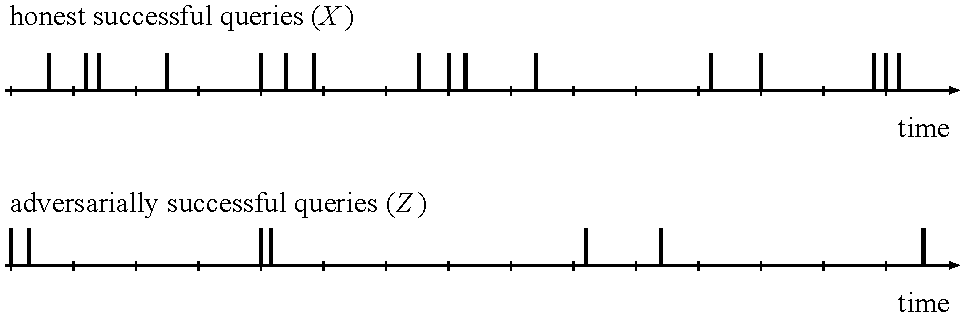
\includegraphics[width=0.8 \columnwidth,keepaspectratio]{figures/x-vs-z.pdf}
    \caption{Honest \emph{vs} adversarially successful queries with a minority adversary.}
    \label{fig.x-vs-z}
\end{figure}

On the other hand, if Eve has the upper hand ($t > n - t$), then the picture looks quite differently.
The longer we wait, the longer the adversarial fork will become, and it will certainly overtake the
honest fork. There is no hope if the adversary has more mining power than the honest parties. This
reaffirms our requirement for the honest majority assumption.

However, this picture is slightly incomplete. While we have argued that Eve will mine fewer blocks
than the honest parties within the window of time in question, any honestly successful queries that are
not convergence opportunities may be wasted into temporary forks. On the contrary, because Eve
is a puppetmaster adversary, if she plays her hand right, her queries are coordinated and always
lead to one consistent chain without forks. Therefore, it is not the honest successful queries
we should be comparing against the adversarially successful queries. Instead, we should be comparing
the \emph{convergence opportunities} against the adversarially successful queries. The full
picture is illustrated in Figure~\ref{fig.x-vs-y-vs-z}. As you can see, even though the honestly
successful queries (labelled $X$ at the top) might be more dense than the adversarially successful queries
(labelled $Z$ at the bottom) due to honest majority ($t < n - t$), it is still possible that
the convergence opportunities (labelled $Y$ in the middle) are fewer than the adversarially successful
queries. In order for the honest parties to win the Nakamoto Race, honest majority is not enough!
In addition to honest majority, the blockchain must be correctly configured (with an appropriately
chosen $T$) so that the convergence opportunities are denser than the adversarial successes.
Of course, because convergence opportunities are always sparser than successful queries
(every convergence opportunity is a successful query, but not vice versa),
if honest majority does not hold, then there is no hope that convergence opportunities are denser
than adversarial successes.

\begin{figure}[h]
    \centering
    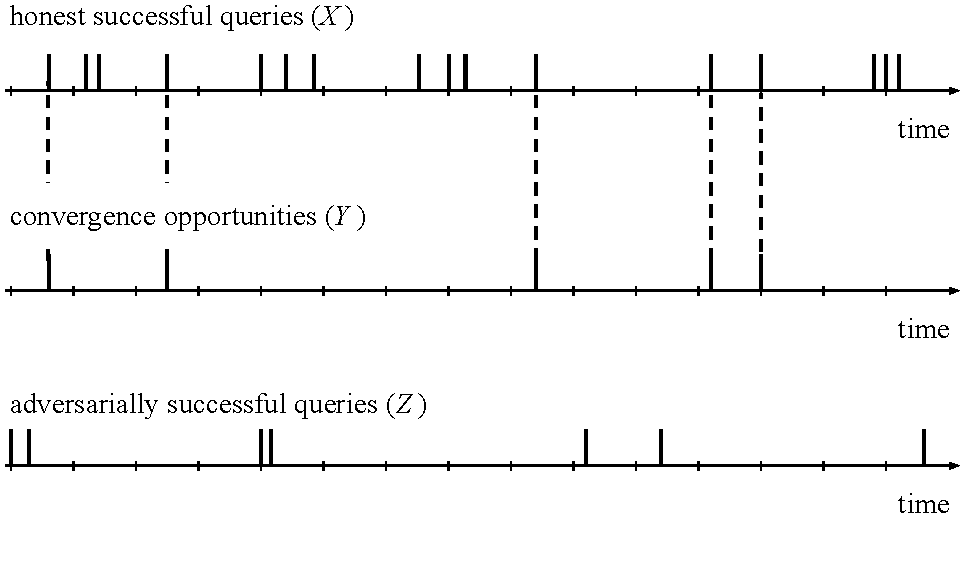
\includegraphics[width=0.8 \columnwidth,keepaspectratio]{figures/x-vs-y-vs-z.pdf}
    \caption{Convergence opportunities \emph{vs} adversarial queries with honest majority
             in a misconfigured blockchain.}
    \label{fig.x-vs-y-vs-z}
\end{figure}

\section{The Fan-Out}

We just observed that honest majority is not enough for our system to be functional. It is not
the honestly successful queries that we must be comparing against adversarially successful queries;
rather, it is the convergence opportunities that we must be comparing against adversarially successful
queries. A misconfigured system, in which the honest parties have more successful queries than the
adversary, but the adversary has more successful queries than the honest parties have convergence
opportunities, can lead to a situation of a \emph{fan-out}\index{Fan Out}.

\begin{figure}[h]
    \centering
    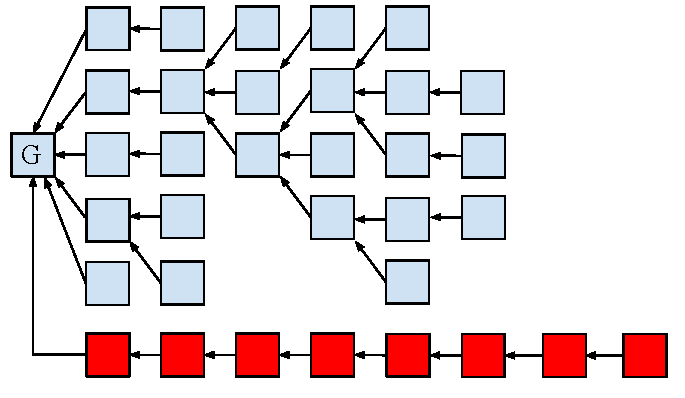
\includegraphics[width=0.8 \columnwidth,keepaspectratio]{figures/fan-out.pdf}
    \caption{A misconfigured blockchain can be subject to fan-outs, even under honest majority.}
    \label{fig.fan-out}
\end{figure}

One such situation is illustrated in Figure~\ref{fig.fan-out}. This system has a target $T$
that is too easy, and so blocks are produced with high probability $p$, more quickly than we
want. As such, the blocktree looks nothing like a blockchain. The honest parties mine the
various blue forks on top. The adversary mines the red fork at the bottom, in secret.
Even though the adversary has only expended $8$ successful queries to build her chain,
the honest parties have expended $25$ successful queries into building their fan-out
structure, whose longest chain is shorter than the adversarially mined chain. The reason
why this situation has occurred is because none of the honest successful queries were
convergence opportunities. Because the minority adversary can concentrate her mining
power into building \emph{one} chain and, contrary to the honest parties, is not subject
to the delay $\Delta$ (remember that we assume she controls all of her minions from one
central puppetmaster), she can win the race against the honest parties even though they
control the majority of compute. Because all but one of the temporary forks among the
honestly mined ones will eventually be thrown out when a convergence opportunity occurs,
all this honest mining power is going to waste.

\section{Chain Quality and Chain Growth}

We spoke about how Common Prefix gives rise to \emph{safety}. Just having our chains
have common prefix does not give \emph{liveness}, however. It is possible that the chains
have simply stopped growing, and no new transactions are ever making it in. In order
for liveness to hold, we need honest transactions to make it into the stable chains
of honest parties. Towards this, we will hope our chains will have two more virtues.

On the one hand, we want honest chains to grow. If chains do not grow at all, then
there is no hope of new transactions making it in. As long as our chain grows
at a positive rate, however, we will have some liveness. The rate at which the
chain of an honest party grows over a period of time if the chain velocity.

\glsxtrnewsymbol[description={chain velocity}]{chain velocity}{$\tau$}\glsadd{chain velocity}
\begin{definition}[Chain Velocity]
  Consider an honest party and his chain $C_1$, $C_2$ at times $r_1 < r_2$ respectively.
  We say the chain has grown with a \emph{velocity}
  $\tau = \frac{|C_2| - |C_1|}{|\chain_{r_2}| - |\chain_{r_1}|}$
  between those times.
\end{definition}

In order to achieve liveness, we will hope that our chain has \emph{chain growth}:
Given enough time, the chain grows with a minimum velocity $\tau$.
% TODO: chain growth picture?

On the other hand, just because the chain has grown does not mean that any honest
transactions are getting confirmed: If the chain has only grown by adversarially mined
blocks, it is possible that the adversary has simply been ignoring the honestly generated
transactions. In order to get ledger liveness, we hope to occassionally see an honestly
mined block in every sufficiently long chain. We call this \emph{chain quality}.

\glsxtrnewsymbol[description={chain quality}]{chain quality}{$\mu$}\glsadd{chain quality}
\begin{definition}[Chain Quality]
  Consider the chunk $\chain[i{:}j]$ of an honest party's adopted chain $\chain$.
  We say that the chunk has chain quality $\mu = \frac{z}{|\chain[i{:}j]|}$, where
  $z$ is the number of honest blocks in $\chain[i{:}j]$.
\end{definition}

In other words, the chain quality metric defines the \emph{proportion} of honest blocks
within an honestly adopted chain. The \emph{chain quality} virtue demands that
sufficient long chain chunks of honest parties have a minimum quality $\mu$. An example
is illustrated in Figure~\ref{fig.chain-quality}. This is an honestly adopted chain $\chain$
which contains both honestly and adversarially generated blocks. Blocks $1, 2, 5, 7, 8$
are adversarially generated, and blocks $\mathcal{G}, 3, 4, 6$ are honestly generated.
This chain has quality $\mu = \frac{4}{9}$. If we just focus on the chunk $\chain[3{:}6]$,
the quality of this chunk is $\mu = \frac{2}{3}$.

\begin{figure}[h]
    \centering
    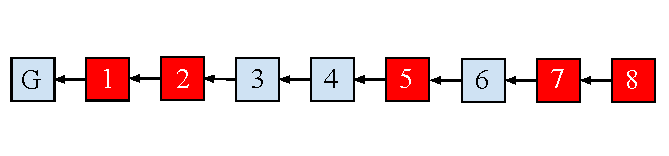
\includegraphics[width=0.7 \columnwidth,keepaspectratio]{figures/chain-quality.pdf}
    \caption{An honesty adopted chain with both honestly and adversarially generated blocks.
             Adversarial blocks are numbered $1, 2, 5, 7, 8$ and shown in red.}
    \label{fig.chain-quality}
\end{figure}

Liveness follows from chain growth and chain quality.
Liveness mandates that an honestly generated transaction is confirmed ``soon''.
When the honest transaction is broadcast into the network, it makes it into every
honest party's mempool (whereas the adversary can ignore it). As soon as any honest
block is mined, the transaction will make it into the block if it has not been
included in a previous block. Due to chain growth, the chain will grow at a minimum
rate of $\tau > 0$. When the chain grows enough, the fresh chain chunk will have a minimum
quality $\mu > 0$, and so will contain at least one honest block. That block will
contain the transaction in question. This is captured in the following theorem:

\begin{theorem}[Chain Growth and Chain Quality $\Rightarrow$ Liveness (informal)]
    If the blocktree satisfies Chain Growth and Chain Quality with positive parameters $\tau$
    and $\mu$ respectively, then the longest chain protocol is live.
\end{theorem}

Notice here the Common Prefix parameter $k$ is a part of our \emph{construction} and is a value
hard-coded into our implementation of the \emph{read} functionality. If we choose this value
wisely, we can prove that the Common Prefix virtue with parameter $k$ is respected. The $\tau$
and $\mu$ parameters are not part of our construction. We will simply calculate these values
when we prove that our chains attain all three virtues.

In summary, chain virtues give rise to ledger virtues. Safety follows from Common Prefix
and liveness follows from Chain Growth and Chain Quality together.

\section{Further Reading}
The two chain virtues of Common Prefix and Chain Quality were first defined in the Bitcoin Backbone paper~\cite{backbone}
by Juan Garay, Aggelos Kiayias and Nikos Leonardos. The Chain Growth virtue was identified in a later paper~\cite{speedsecurity}
by Aggelos Kiayias and Giorgos Panagiotakos. The ledger virtues of safety and liveness have been adapted, with appropriate
modification, from older literature from the 1980s and 1990s in the context of two problems known as the Byzantine Generals
Problem and the Byzantine Agreement Problem. These two problems are very related to the type of problem that blockchains
are trying to solve. The Byzantine Generals Problem was originally studied in a seminal 1982 paper~\cite{lamport} by Leslie Lamport,
Robert Shostak, and Marshall Pease.
% TODO: add citations to these

\section{Problems}

TBD
